% !TEX root = ../../../main.tex
%

\section{Analisi}
Prima di procedere con la prima parte del progetto, è necessario analizzare collettivamente
le planimetrie ed i requisiti indicati. Si sceglie di iniziare dai requisiti necessari a soddisfare
gli utenti finali di questo progetto, ovvero i dipendenti aziendali (ed in genere chiunque debba collegarsi
alla rete in questione). Dal punto di vista del cablaggio strutturato, il vincolo è dato principalmente dalle
postazioni e dalle apparecchiature da collegare alla rete cablata, in quanto richiederanno un numero minimo
ben preciso di prese a muro, necessarie non solo a garantire il loro collegamento, ma anche a mantenere una ridondanza
sufficientemente elevata. Questo si rivela utile al fine di scongiurare interventi eccessivamente lunghi,
costosi ed invasivi ad ogni danneggiamento di una linea od un apparato di rete.

\subsection{Conteggio delle prese utente}

Si è effettuato il conteggio delle prese (del piano terra) secondo la seguente tabella:

\begin{table}[h]
  \begin{adjustbox}{center}
    \begin{tabular}{@{}lclr@{}}
      \toprule
      Stanza                         & Numero stanze       & Uso presa                                          & Numero prese \\ \midrule
      \multirow{8}{*}{Hall}          & \multirow{8}{*}{1}  & Telefonia (scrivania)                              & 2            \\
                                     &                     & Citofono (scrivania)                               & 1            \\
                                     &                     & Citofono (muro)                                    & 1            \\
                                     &                     & Computer (scrivania)                               & 2            \\
                                     &                     & Access point                                       & 1            \\
                                     &                     & Prese ridondanti/espansioni (scrivania)            & 4            \\
                                     &                     & Apricancello e azionamenti esterni (muro)          & 2            \\
                                     &                     & Prese ridondanti (muro)                            & 1            \\ \midrule
      \multirow{7}{*}{Sala riunioni} & \multirow{7}{*}{1}  & Connessione laptop partecipanti (tavolo)           & 16           \\
                                     &                     & Telefonia VoIP per (video)conferenze (tavolo)      & 2            \\
                                     &                     & Telefonia standard (tavolo)                        & 2            \\
                                     &                     & Access point (visitatori + rete interna, separati) & 2            \\
                                     &                     & Proiettore o lavagna multimediale (muro)           & 1            \\
                                     &                     & Computer per presentazioni (muro)                  & 1            \\
                                     &                     & Prese ridondanti (muro)                            & 2            \\ \midrule
      \multirow{3}{*}{Ufficio}       & \multirow{3}{*}{10} & Telefonia                                          & 1            \\
                                     &                     & Workstation                                        & 1            \\
                                     &                     & Prese ridondanti                                   & 1            \\ \bottomrule
    \end{tabular}
  \end{adjustbox}
  \caption{\label{tab:prese-terra} Conteggio delle prese del piano terra.}
\end{table}

\begin{figure}[ht]
  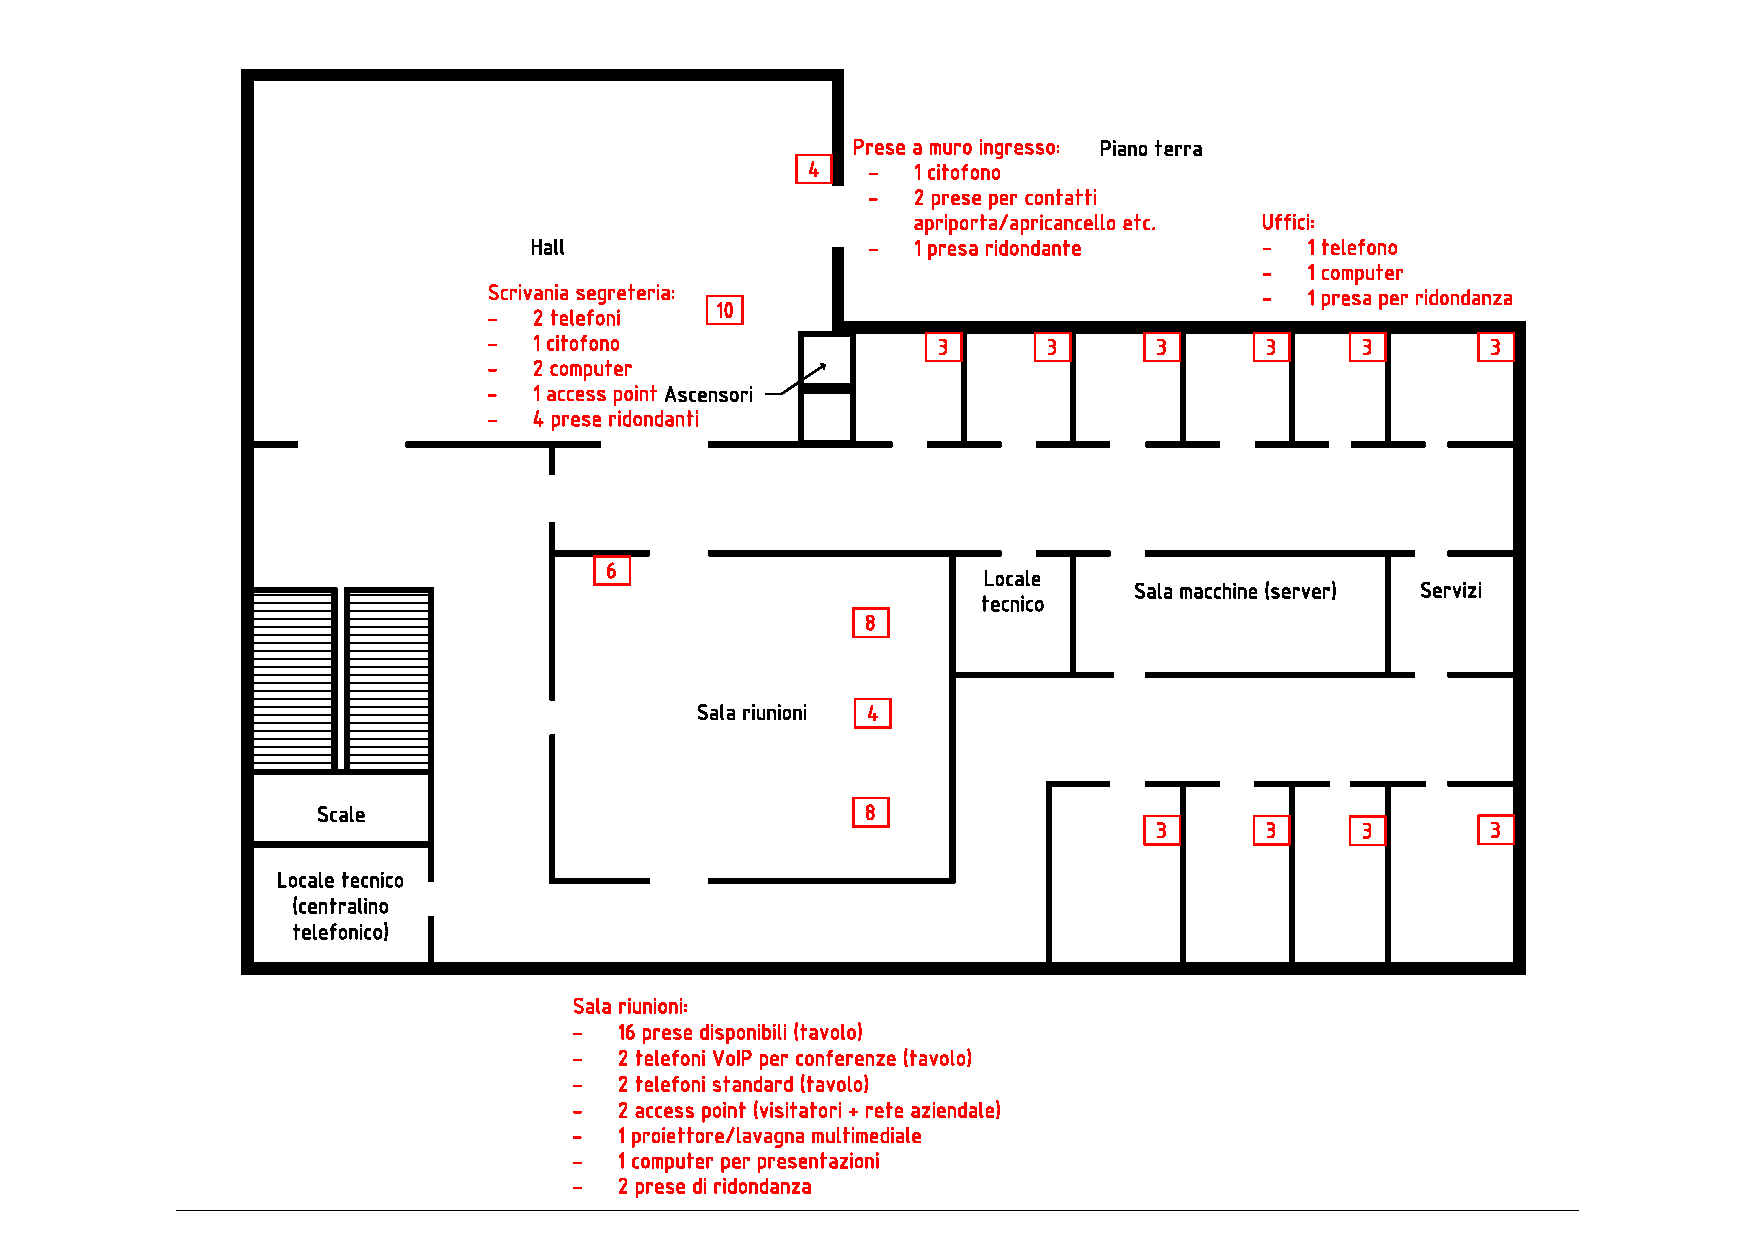
\includegraphics[width=\textwidth]{planimetrie-pianoterra-prese}
  \caption{Planimetria del piano terreno, comprensiva di posizionamento e conteggio delle prese multiuso.}\label{fig:planimetria-terreno-prese}
\end{figure}

\newpage
Per il primo piano ed i superiori, il conteggio è il seguente:

\begin{table}[ht]
  % \begin{adjustbox}{center}
  \begin{tabular}{@{}lclr@{}}
    \toprule
    Stanza                   & Numero stanze       & Uso presa        & Numero prese \\ \midrule
    \multirow{3}{*}{Ufficio} & \multirow{3}{*}{27} & Telefonia        & 1            \\
                             &                     & Workstation      & 1            \\
                             &                     & Prese ridondanti & 1            \\ \bottomrule
  \end{tabular}
  % \end{adjustbox}
  \caption{\label{tab:prese-1} Conteggio delle prese del primo piano e i superiori.}
\end{table}

\begin{figure}[ht]
  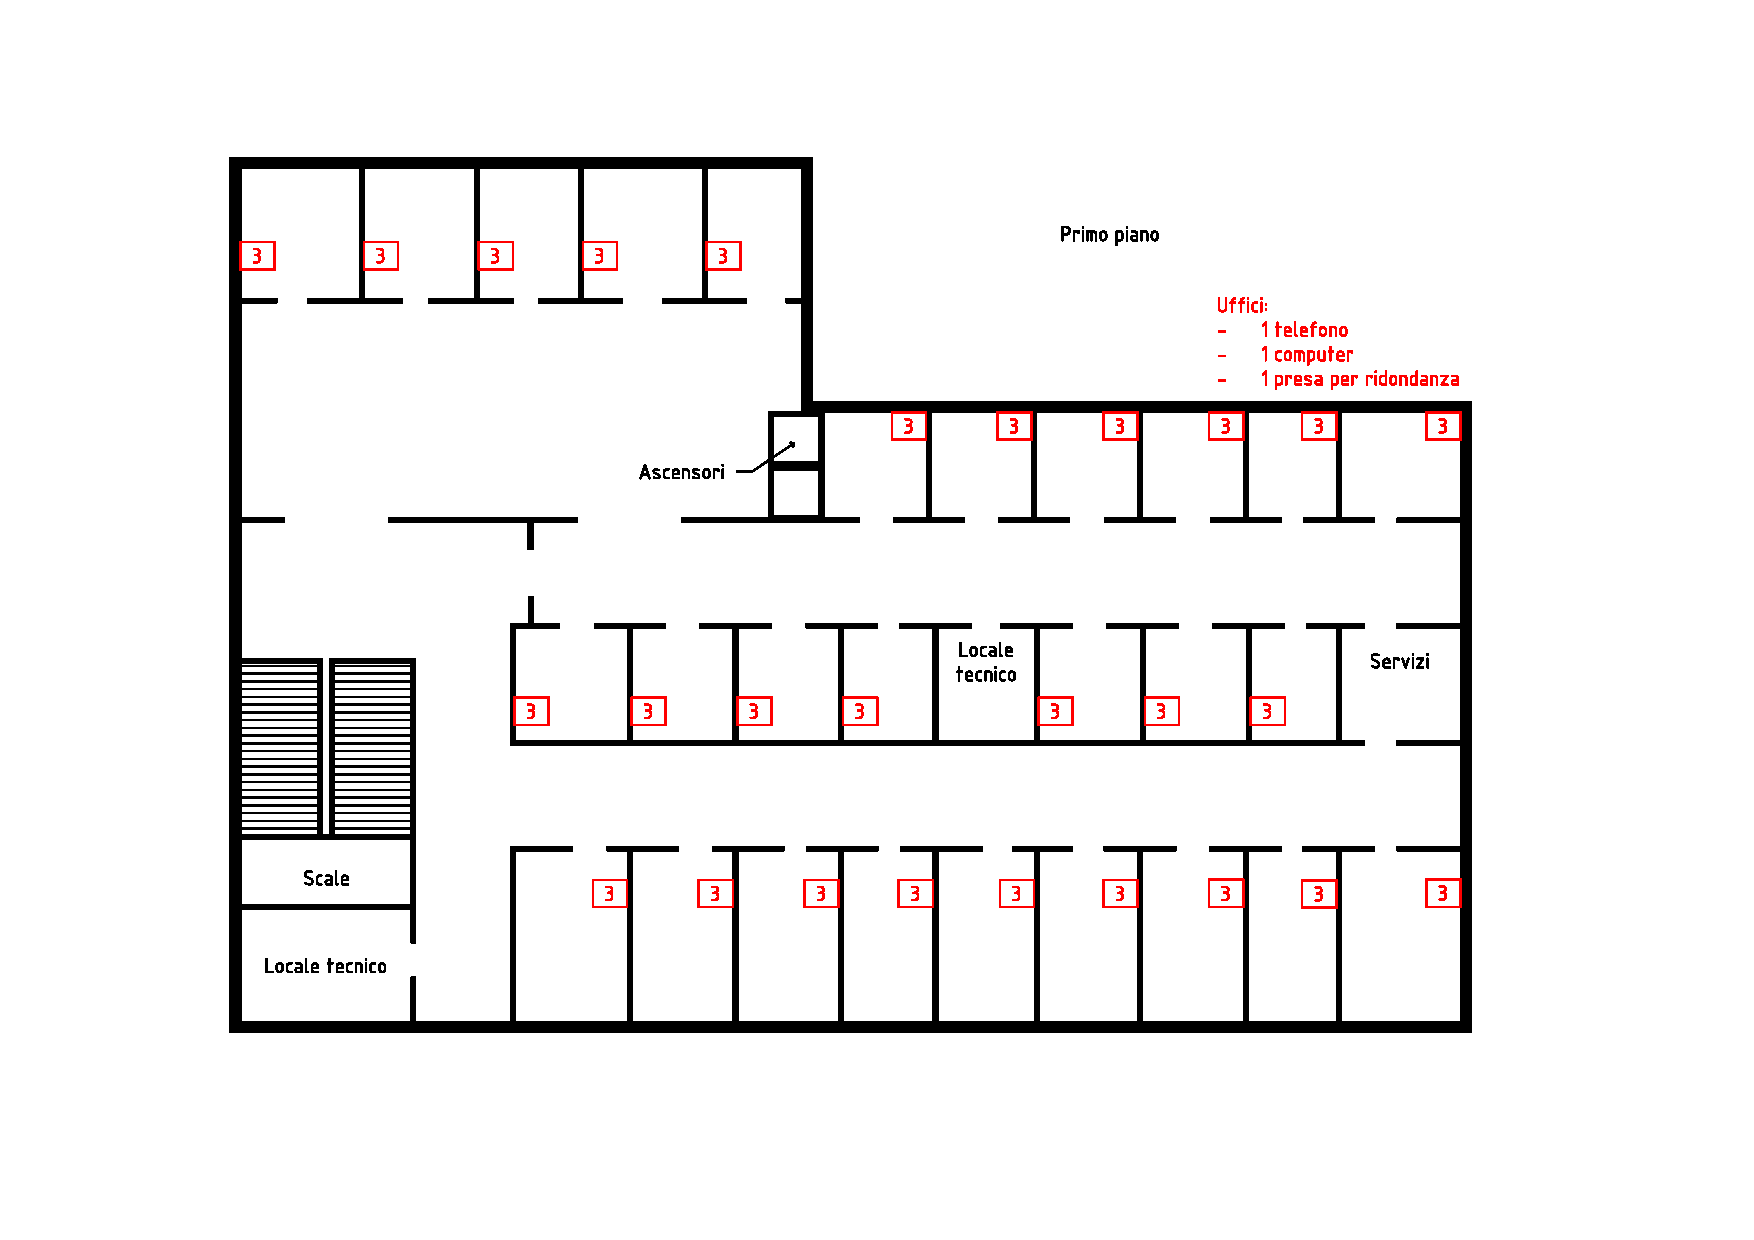
\includegraphics[width=\textwidth]{planimetrie-piano1-prese}
  \caption{Planimetria del primo piano e dei successivi, comprensivi di posizionamento e conteggio delle prese multiuso.}\label{fig:planimetria-1-prese}
\end{figure}

Riassumendo, saranno necessarie \num{70} prese al piano terreno, e \num{81} per ogni piano al di sopra.
Questo porta il numero totale di prese a 394, per poter servire 118 uffici, ognuno con un collegamento alla rete locale,
un collegamento fonia ed una presa ridondante o configurabile in caso di necessità. A questi si aggiungono 16 postazioni
sul tavolo della sala riunioni ed una buona disponibilità di connessioni nella hall, la quale potrebbe necessitare di due telefoni,
uno o più computer e svariate prese libere per il controllo di dispositivi come citofoni, meccanismi apricancello e sistemi di
allarme.

L'aggiunta di una presa ridondante in ogni postazione ovviamente aggiunge un peso non indifferente al conteggio totale,
ma si ritiene il beneficio di una immediata possibilità di riconfigurazione in caso di guasto, o l'aggiunta/spostamento di apparecchiature
di test giustifichi questa aggiunta. Ovviamente certe industrie non godrebbero a pieno di una simile configurazione, ma si pensi, ad esempio, al
dipartimento di ricerca e sviluppo di un'azienda specializzata nella costruzione di dispositivi elettronici: una presa aggiuntiva consentirebbe
ad un dipendente di poter portare alla sua postazione una qualsiasi apparecchiatura di test, come ad esempio un oscilloscopio,
e connetterla alla rete per poter effettuare delle prove automatizzate durante lo sviluppo del firmware per questo dispositivo.
Difficilmente una simile apparecchiatura avrà funzionalità di controllo remoto wireless. È invece molto comune trovare connettori RJ45 per il collegamento Ethernet.

\begin{quotation}
  \color{gray}
  Questo è un esempio basato semplicemente su passate esperienze di stage, in cui vi era la necessità di effettuare dei test
  automatizzati su dei dispositivi in prova. La presenza abbondante di connessioni di rete cablate ha consentito la riconfigurazione
  di una parte di un laboratorio.
\end{quotation}
